%\documentclass[spanish]{beamer}

\documentclass{beamer}
\usepackage{pgf,pgfpages}
%\pgfpagesuselayout{4 on 1}[letterpaper,landscape,border shrink=0.5in]
\usepackage{algorithm,algorithmic}
%\usepackage{algorithm,algorithmicx}
%\usepackage[noend]{algpseudocode}
\usepackage{listings}
\lstset{basicstyle=\ttfamily,
	showstringspaces=false,
	commentstyle=\color{red},
	literate={á}{{\'a}}1
	{ã}{{\~a}}1
	{é}{{\'e}}1
	{ó}{{\'o}}1
	{í}{{\'i}}1
	{ñ}{{\~n}}1
	{¡}{{!`}}1
	{¿}{{?`}}1
	{ú}{{\'u}}1
	{Í}{{\'I}}1
	{Ó}{{\'O}}1
}

\usepackage{beamerthemesplit}
\usepackage{color}
\usepackage[utf8]{inputenc}
\usepackage[spanish]{babel}
%\usepackage[latin1]{inputenc}
%\usepackage[pdftex]{graphicx}
%\usepackage{algorithm}
%\usepackage{algorithmic-C}
%\usepackage{algorithmic}
\usepackage{amsthm}
\usepackage{multicol}
\usepackage{multirow}
\usepackage{fancyvrb,relsize}
\usepackage{hhline}
\usepackage{tikz}
\usetikzlibrary{trees, shapes, calc}
\newcommand{\inputTikZ}[2]{%
	\scalebox{#1}{\input{#2}}
}

\usetheme{Warsaw} %Gueno
%\usetheme{Darmstadt} %OK!
% \usetheme{Frankfurt} %OK!
%\usetheme{Goettingen}
%\usetheme{Dresden}
%\usetheme{JuanLesPins} %OK!!
%\usetheme{Marburg}
%\usetheme{Montpellier}
%\usetheme{Rochester} %sobrio
%\usetheme{Singapore}
%\usetheme{Szeged}

%\usecolortheme{albatross}
%\usecolortheme{seahorse}
%\usecolortheme{beetle}
%\usecolortheme{crane}
%\usecolortheme{dolphin}
%\usecolortheme{dove}
%\usecolortheme{fly}
%\usecolortheme{lily} %Gueno
\usecolortheme{orchid}%Gueno
%\usecolortheme{rose}
%\usecolortheme{seagull}
%\usecolortheme{whale}


\DefineVerbatimEnvironment%
      {VerbatimNN}%
      {Verbatim}%
      {fontsize=\relsize{-1}}
\DefineVerbatimEnvironment%
      {VerbatimNNN}%
      {Verbatim}%
      {fontsize=\relsize{-2}}

\DefineVerbatimEnvironment%
      {VerbatimPseudo}%
      {Verbatim}%
      {numbers=left, fontsize=\relsize{-1}}
\DefineVerbatimEnvironment%
      {VerbatimPseudoReduced}%
      {Verbatim}%
      {numbers=left, fontsize=\relsize{-2}}
\DefineVerbatimEnvironment%
      {VerbatimPseudoReduced2}%
      {Verbatim}%
      {numbers=left, fontsize=\relsize{-3}}
\DefineVerbatimEnvironment%
      {VerbatimC}%
      {Verbatim}%
      {commandchars=@ªº, numbers=left, fontsize=\relsize{-1}}
\DefineVerbatimEnvironment%
      {VerbatimReducedC}%
      {Verbatim}%
      {commandchars=@ªº, numbers=left, fontsize=\relsize{-2}}
\DefineVerbatimEnvironment%
      {VerbatimReduced2C}%
      {Verbatim}%
      {commandchars=@ªº, numbers=left, fontsize=\relsize{-3}}



%\AtBeginSubsection[]
%{
% \begin{frame}
% \frametitle{Sinopsis}
% Aqui decides: cada seccion y subseccion:
% \tableofcontents[currentsection,currentsubsection]
 %O solamente la seccion (Solo uno de ellos)
%\tableofcontents[currentsection]
% \end{frame}
%}

% Si quieres que todo por default aparezca de poco en poco
% descomenta esta linea
%\beamerdefaultoverlayspecification{<+->}

\setbeamertemplate{footline}{\hfill\insertframenumber/\inserttotalframenumber}
\setbeamertemplate{navigation symbols}{}

\setbeamercovered{transparent}

\title{ELO320 - Estructuras de Datos y Algoritmos\\Introducción a C\\Funciones y Arreglos}
%\subtitle{Ingeniería Civil Telemática UTFSM}
\author{Dr. Nicolás Gálvez R.\\{\small nicolas.galvez@usm.cl}}
\institute{Ing. Civil Telemática - Departamento de Electrónica}
\titlegraphic{
\includegraphics[scale=.18]{images/logoutfsm}}
\date{2do Semestre 2022}

\begin{document}

\frame{\titlepage}

%\section*{Sinopsis}
%\frame{  \frametitle{Sinopsis}\tableofcontents[pausesections]}
%
%

\section{Funciones}
\begin{frame}[fragile]{Funciones en C}
\begin{itemize}
	\item Encapsula código.
	\item Permite reutilizar código.
	\item Se pueden compilar por separado.
	\item Retorna siempre un tipo de dato específico. 
\end{itemize}
\end{frame}

\begin{frame}[fragile]{Funciones en C}
\begin{itemize}
	\item Se puede separar interfaz (prototipo) de implementación.
	\item \textbf{Interfaz (prototipo):} Sólo define existencia y formato de función. Suficiente para ser invocada.
	\begin{exampleblock}{C}
	\begin{lstlisting}[language=C, basicstyle=\tiny]
//tipo_retorno funcion(parametros con o sin nombre);
float potencia(float a, float b);
//....

calculo = x * potencia(y, 2.5);
\end{lstlisting}\end{exampleblock}
	\item \textbf{Implementación:} Define implementación de código de función.
	\begin{exampleblock}{C}
\begin{lstlisting}[language=C, basicstyle=\tiny]
/*tipo_retorno funcion(parametros con nombre) {
*	Implementacion...
}*/

float potencia(float a, float b) {
	return power(a,b);
}
\end{lstlisting}\end{exampleblock}
\end{itemize}
\end{frame}

\begin{frame}[fragile]{Funciones en C}
\begin{itemize}
	\item Si se utiliza solamente la implementación, está tiene que estar definida \textbf{antes} de la función que la invoca.
	\item Si se utiliza el prototipo, es éste el que debe estar defindo \textbf{antes} de la función que la invoca.
	\item Prototipo + Implementación: libertad de ubicación de la implementación.
\end{itemize}
\end{frame}

\begin{frame}[fragile]{Funciones en Python}
\begin{itemize}
	\item \textbf{Python} sólo permite implementación, no prototipos.
\begin{block}{Python}
	\begin{lstlisting}[language=Python, basicstyle=\scriptsize]
def nombre_funcion(parametros):
    #...Implementacion
    return <expresion>
	\end{lstlisting}
\end{block}
	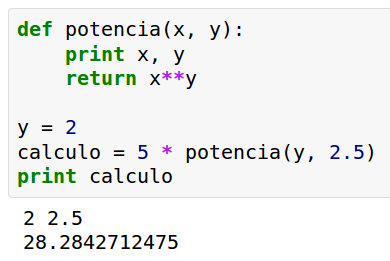
\includegraphics[width=.7\linewidth]{images/funcion-python.png}
\end{itemize}
\end{frame}



\subsection{Macros, Constanes, Ámbito, Var. Global y Var. Local}

\begin{frame}[fragile]{Macro}
Una macro es un valor o conjuntos de instrucciones constantes que se definen a nivel de preprocesamiento. No es una variable y no puede ser modificada. 

\begin{exampleblock}{C}
\begin{lstlisting}[language=C, basicstyle=\scriptsize, escapeinside={|}{|}]
#include<stdio.h>
#define MACRO 10

int main(){
	int a = 5;
	printf("|\%|"s\n", a*MACRO);
}
\end{lstlisting}\end{exampleblock}
\end{frame}


\begin{frame}[fragile]{Constante}
Una variable constante es aquella que se declara con el keyword \textbf{const}, e implica que ésta no puede ser modificada. Tiene todo el resto de las propiedades de una variable común.

\begin{exampleblock}{C}
\begin{lstlisting}[language=C, basicstyle=\scriptsize, escapeinside={|}{|}]
#include<stdio.h>

int main(){
	const int a = 5;
	a = 10; //¿Cómo actúa el compilador?
	printf("|\%|"d\n", a);
}
\end{lstlisting}\end{exampleblock}
\end{frame}

\begin{frame}[fragile]{Ámbito (Scope)}
Las funciones (includa main) definen el alcance de las variables, llamado \textbf{ámbito}, vale decir, el segmento en el cual existen y pueden ser usadas $\rightarrow$ entre \{ y \}.

\begin{exampleblock}{C}
\begin{lstlisting}[language=C, basicstyle=\scriptsize, escapeinside={|}{|}]
#include<stdio.h>

void saludo(){ // var i sirve sólo dentro de función saludo.
	int i = 5;
	printf("Hola alumno numero |\%|d", i);
}

int main(){// var a sirve sólo dentro de función main. 
	int a = 10;
	saludo();
	printf("|\%|"d\n", a);
	return 0;
}
\end{lstlisting}\end{exampleblock}
\end{frame}

\begin{frame}[fragile]{Variable local}
Una variable local, es aquella que está definida dentro de un ámbito de terminado, vale decir, una función y/o estructura de control. 

\begin{exampleblock}{C}
\begin{lstlisting}[language=C, basicstyle=\scriptsize, escapeinside={|}{|}]
#include<stdio.h>

int main(){// var a sirve sólo dentro de función main. 
	int a = 10;

	if(a==10){
		int b = 1;
		printf("|\%|d |\%|d\n", a, b);
	}
	// ¿Qué pasa con la variable b?
	printf("|\%|d |\%|d\n", a, b); 

	return 0;
}
\end{lstlisting}\end{exampleblock}
\end{frame}


\begin{frame}[fragile]{Variable Global}
Una variable global, es aquella que está definida fuera de cualquier ámbito. Puede ser llamada, modificada y utilizada desde cualquier ámbito, siempre y cuando no exista una variable local con el mismo nombre. 

\begin{exampleblock}{C}
\begin{lstlisting}[language=C, basicstyle=\scriptsize, escapeinside={|}{|}]
#include<stdio.h>

int a=1; //global
int b=2; //global

int main(){
	int a = 10; //local
	b++;
	printf("|\%|d |\%|d\n", a, b);//¿Qué imprime? 
	return 0;
}
\end{lstlisting}\end{exampleblock}

En python, no se pueden modificar variables globales dentro de una función.
\end{frame}

\section{Arreglos}
\begin{frame}[fragile]{Arreglos y Strings}
\small
\begin{itemize}
	\item \textbf{Arreglo:} Tipo estructurado consistente en conjunto homogéneo y ordenado de elementos.
	\item Se identifican por su posición relativa mediante un \emph{índice} encerrado con paréntesis cuadrados (parte de índice 0).
	\begin{lstlisting}[language=C,basicstyle=\scriptsize,escapeinside={|}{|}]
//Arreglos estáticos (se liberan al terminar 
// el ámbito donde fueron declaradas):
int foo[10]; //10 enteros creados en foo.
foo[3] = 7; //A cuarto elemento se asigna un 7.
	\end{lstlisting}
	
	\item \textbf{String:} Arreglo de caracteres.
	\begin{lstlisting}[language=C,basicstyle=\scriptsize,escapeinside={|}{|}]
// Los string se delimitan con caracter '\0' 
// (requiere espacio de 1 char):
char nombre[10] = "Juan"; //String de largo máximo 10. 
nombre[1] = 'e'; //Qué hace? 
printf("|\%|s\n", nombre);
	\end{lstlisting}

	\item Veremos más sobre strings la próxima clase. 	
\end{itemize}
\end{frame}

\begin{frame}[fragile]{Arreglos Multidimensionales e Inicialización}
Al igual que con las listas de Python, pueden definir arreglos multidimensionales.\\

Además los arreglos pueden ser inicializados utilizando \{ y \}.
\begin{exampleblock}{C}
\begin{lstlisting}[language=C,basicstyle=\scriptsize,escapeinside={|}{|}]
#include<stdio.h>

int main(){
	char nom[10] = "Camilo";
	char a[5][20] = {"Juan", "Francisco", "Pedro"};	
	int b[3][3] = {{1,2,3}, {4,5,6}, {7,8,9}}, i, j;

	for(i=0;i<3;i++){
		for(j=0;j<3;j++) //¿Qué pasó con las llaves? 
			printf("|\%|d ", b[i][j]);
		printf("\n");
	}
}
\end{lstlisting}
\end{exampleblock}
\end{frame}

\begin{frame}[fragile]{Recorrer un arreglo}
Podemos utilizar cualquiera de las estructuras de control iterativas para recorrerlos. 
\begin{exampleblock}{C}
\begin{lstlisting}[language=C,basicstyle=\scriptsize,escapeinside={|}{|}]
#inclede<stdio.h>

int main(){
	int i;
	float a[5];
	
	for(i=0;i<5;i++){
		float val; //¿Cuántas veces nace y muere val?
		scanf("|\%|f", &val);
		a[i]=val;
	} //¿Cómo reducir este código?

}
\end{lstlisting}
\end{exampleblock}
\end{frame}

\begin{frame}[fragile]{Recorrer un arreglo}
Practiquen con los siguientes ejercicios:
\begin{itemize}
\item Calcular el factorial de un número dado.
\item Ordenar de mayor a menor un arreglo de una dimensión.
\item Encontrar el mayor elemento en un arreglo de dos dimensiones.
\item Calcular el promedio de los elementos en un arreglo bidimensional.
\item Imprimir en orden inverso los elementos de un arreglo. 
\item Imprimir todas las letras mayúsculas y minúsculas del alfabeto (ver Código ASCII).
\end{itemize}

\end{frame}


%\begin{frame}[fragile]{Operaciones sobre Strings}
%Para operaciones sobre arreglos de caracteres, se debe incluir la biblioteca \textbf{cstring}.\\
%
%\begin{itemize}
%\item \textbf{C/C++}
%\end{itemize}
%\begin{lstlisting}[language=C++]
%
%#include <cstring>
%//...
%char str1[10] = "hola ";
%char str2[10] = "mundo";
%// Imprime 5
%std::cout<<strlen(str1)<<std::endl; 
%// Imprime "hola mundo"
%std::cout<<strcat(str1,str2)<<std::endl; 
%strcpy(str1,str2);
%// Imprime "mundo"
%std::cout<<str1<<std::endl; 
%\end{lstlisting}
%\end{frame}
%
%\begin{frame}[fragile]{Operaciones sobre Strings}
%\begin{itemize}
%\item \textbf{Equivalentes en Python}
%\begin{lstlisting}[language=Python]
%#...
%str1 = "hola "
%str2 =  "mundo"
%# Imprime 5
%print(len(str1))
%# Imprime "hola mundo"
%print(str1 + str2)
%str1 = str2
%# Imprime "mundo"
%print(str1)
%#...
%\end{lstlisting}
%\end{itemize}
%\end{frame}
%
%\begin{frame}[fragile]{Tipos de Datos Abstractos - Estructuras}
%\begin{itemize}
%	\item Conjunto (posiblemente) heterogéneo de elementos de datos (e.g.: estructuras y clases).
%	\item Cada elemento individual (campo, miembro o atributo) identificado con un nombre. 
%	\item Encapsulamiento de información.
%	\item Ejemplo:
%	\begin{lstlisting}[language=C++]
%struct empleado {
%    char nombre[40];
%    char ap_paterno[40];
%    char ap_materno[40];
%    float sueldo;
%};
%//...
%empleado e1, e2;
%
%//Acceso a atributos con operador '.'
%e1.sueldo = 550000.00;
%strcpy(e1.nombre, "Juan");
%	\end{lstlisting}
%\end{itemize}
%\end{frame}



\end{document}
